% CHAPTER_BEGIN
\section{Ajira Framework: Research Report}

\subsection{Introduction}

The \textit{ajira} project represents a custom made framework for writing mainly HPC data applications. It is built as a framework on top of IPL (Ibis Portability Layer - communication layer) adopting a master-slave architecture. The master is basically another slave that hast the extra requirement to setup the communication and start splitting the job between all the nodes (slaves). Thus, we do not have to install and configure anything as a separate platform and then use a special API to run jobs/tasks on top of that platform (i.e such as using Hadoop). With other words, what we need to run an application is the \textit{ibis-server} (it is embedded inside the \textit{ajira} framework so we can run it from there and have our node communication layer) and, of course, a program that uses \textit{ajira} to compute some data. Usually, the program does not have to be divided into a master and slave architecture. We can only use \textit{ajira} framework to write the master section. The slaves' behavior is automatically dictated by the list of actions we add in the code, inside the job's description. For testing my experimental changes on \textit{ajira} I have run an application built with \textit{ajira} framework that sorts large data-sets of RDF triples. To build and run this entire setup (\textit{ajira} + \textit{sorting application}) I have used the git repository for code deployment on DAS4 and a self written ant file \cite{build_file} to build the application into a .jar bundle package (a package that embeds inside all the necessary dependencies, including the \textit{ajira.jar} package built with the default ant file). Next, to run the \textit{sorting application} on DAS4 was a simple \textit{prun} command execution (see next section).

% 
\subsection{Deployment \& execution on DAS4}

For \textit{ajira's} and \textit{sorting application's} main-code deployment on DAS4 you will first need access to their git repositories \cite{arch_repo}, \cite{qpie_repo}. After that, just simply clone the repositories in your home DAS4 directory and be sure that you are located in the benchm\_master branch. For the entire list of steps that you have to follow in order to run/execute this setup on multiple nodes, read next.
\newline
\newline
\textbf{Steps for running the \textit{sorting application} on multiple DAS4 cluster nodes:}
\begin{enumerate}
	\item Deploy \textit{ajira} and the \textit{demo sorting application} projects in your home DAS4 directory. Each project already has all the dependencies packages and ant files necessary for automatic build. 
	\item Build \textit{ajira} project using its ant build file: 'ant build-jar' 
	\item Copy the \textit{ajira.jar} package in the \textit{/lib} directory of the \textit{sorting app}
	\item Build \textit{sorting app} project using its ant build file \cite{build_file}: 'ant build-jar' (will create a .jar bundle package that we use to execute its main class - BenchmarkSorting - on DAS4; the .jar is placed by default in the \textit{/jar} directory -- for any change you wish to do look for the parameters inside the ant file)
	\item Configure \textit{ibis-server} parameters (port, enable events, etc) from inside \textit{ajira's} ant build file 
	\item Start \textit{ibis-server} on the DAS4 head-node from the \textit{ajira} project directory: 'ant ibis-server' (note the address and port that is using)
	\item Run/execute the bundle package on DAS4 using the script example \cite{run_on_das4} -- change the parameters for your own needs.
\end{enumerate}

% 
\subsection{Workflow example: how \textit{ajira} can be used to sort RDF triples}

In this section I will explain how the \textit{ajira} framework works on 'crunching' data, using as a workflow example the RDF triples' \textit{distributed sorting} implemented in the \textit{sorting example application}. To begin with, the process of sorting can be split in 3 steps: (1) read and sort the RDF triples; (2) send-receive communication; (3) merge and write the RDF triples in files;

The main data structure used in all three steps is the 'Bucket' -- an in-memory buffer that is filled up with triples of which hash keys are equal to the bucket's identifier. When the buffer limit size is exceeded, all its content gets sorted and cached on the hard-disk (in files). Thus, when we refer to the 'Bucket' we usually mean both the in-memory buffer and the hard-disk stored files (if data hits the disk). Each time the files' number increases above a fixed limit, a thread is started to merge them 2-by-2 up until their number gets below. All the information about the files (metadata such as names, first elements, size, etc) is kept inside the Bucket -- we need them at the time we transfer the triples or when we write the resulted set back. By default, each node keeps 1 bucket in the memory for every other node (remote-buckets), including itself (local-bucket). So, there are by default N buckets on each node, where N = number of nodes; a new feature allows you to use more than 1 bucket per node (NPARTITIONS\_PER\_NODE parameter, which by default is 1). The creation and initialization of a bucket (create, get, release, etc) is controlled by the 'Buckets' wrapper class.

% 
\subsubsection*{(1) Read and sort the RDF triples}

First, the data set (compressed or not) gets split into file partitions of almost the same sizes, each one being assigned to one node for further reading. The split of the data set is done by the ReadFromFiles action, which creates FileCollections of a minimumFileSplitSize. Next, the FileLayer of each node reads the triples from its assigned partitions -- the FileCollections (a set of path names representing the location of the files that were partitioned) -- and inserts them into the corresponding local/remote bucket (where the triple's hash key equals to the node's bucket id). If a bucket gets full with triples, its content is sorted using the java's default MergeSort algorithm and cached on disk. All the information/metadata about caching the content on the disk is stored inside the Bucket object model for further use. When there is no more data left to read from a partition, the node broadcasts a signal, alerting that the remote-buckets are ready to get transferred (this means that the send-receive start is dependent on the size of the file partition). See Figure~\ref{fig:diag1} for a better understanding. So, at this point, the send-receive step begins -- triples are transferred from the remote-buckets to their assigned nodes (i.e. on node Y, its remote-bucket for node X has triples assigned to X \textit{=>} triples from Y's remote-bucket will be transferred to X's local-bucket).

\begin{figure}
\centering
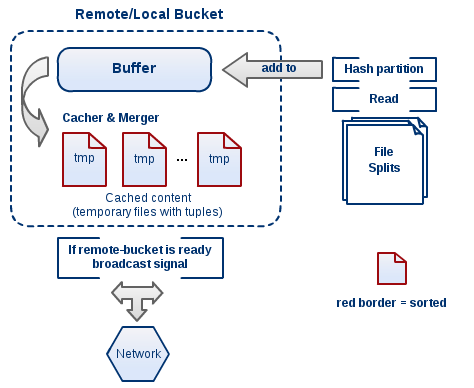
\includegraphics[scale=0.6]{diag1}
\caption{Read and sort - remote \& local buckets structure}
\label{fig:diag1}
\end{figure}

% 
\subsubsection*{(2) Send-receive communication}

When a signal alert for a bucket ready for transfer is received by a node (\textit{receiver}), a corespondent request for fetching triples from it is sent back to the \textit{sender}. Then, the \textit{sender} registers that request and, whenever the remote-bucket has the available data (MIN\_SIZE\_TO\_SEND) for transfer, removes a chunk and sends it to the \textit{requester}. Next, the \textit{recipient} adds that chunk into its local-bucket and \textit{sends} a request for another fetch. As long as on the other side (\textit{sender's} side) the remote-bucket still contains triples, the \textit{receiver} will have chunks get transferred in its local-bucket. If there are no more RDF triples inside of it, the remote-bucket is released and the transfer's metatada are cleaned/removed. But, before that, a last signal that marks the end of the transfer is sent to the \textit{recipient}, which flags its local-bucket with \textit{finished} -- meaning that is ready for merge \& write. In Figure~\ref{fig:diag2} we show very briefly the workflow of the send-receive communication. The chunk removal, in the worst case when triples are getting cached on the disk, has to extract all the minimum triples from the in-memory buffer and the cached files (in sorted order) up until it fills the chunk. Is necessary to do that because we expect to receive sorted data on the \textit{recipient} side. Otherwise, basically, it sends a chunk directly from the in-memory buffer, but after it applies the sort.

\begin{figure}
\centering
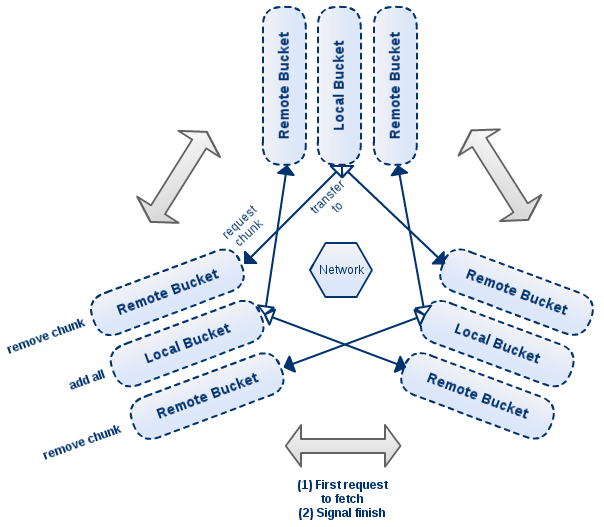
\includegraphics[scale=0.6]{diag2}
\caption{Transfer to correspondent nodes - send-receive communication}
\label{fig:diag2}
\end{figure}

% 
\subsubsection*{(3) Merge and write the RDF triples in files - results output}

After all the triples got moved from the remote-buckets (previous step is finished), the final step is all about merging the local-bucket's in-memory buffer with its cached content (the files from the hard disk, in case data hits the disk). This task is done by the same method (\textit{removeChunk()}) that removes chunks from a bucket. Now it stands for fetching data from the local-bucket whenever the bucket-iterator is called for writing data. In the end, the result at each node is represented by one sorted file with RDF triples (only if we let the default number, equal with 1, of buckets per node). This step is represented by Figure~\ref{fig:diag3}.

\begin{figure}
\centering
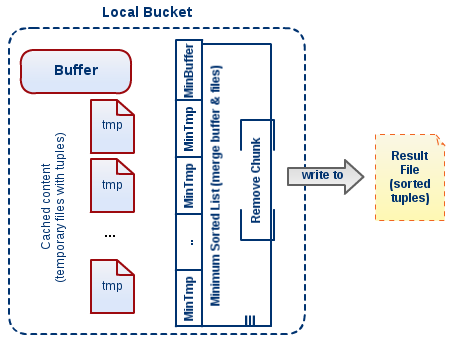
\includegraphics[scale=0.6]{diag3}
\caption{Merge and write}
\label{fig:diag3}
\end{figure}

\pagebreak

% 
\subsection{Execution-time}

Testing configuration: 
\begin{itemize}
	\item \textbf{Cluster-Node}: 1 Node @ DAS4, 16 x QuadCore Intel Xeon CPU E5620 @ 2.4GHz 
	\item \textbf{Number of Nodes}: 8, 12, 16
	\item \textbf{Dataset sizes}: 21, 38, 62, 149 GB
	\item \textbf{Split sizes}: 256MB, 1GB, 2GB, 4GB
	\item \textbf{Common setups}: 512MB buffer size, available to transmit on 128MB (1/4 of buffer size), 8 concurrent tuple senders
\end{itemize}

Test - 8 nodes
\newline \newline
\renewcommand{\arraystretch}{1.2}
{\footnotesize\tt
\begin{tabularx}{\linewidth}{c|c|c|c|c|c|c|c|c|c|l}
\cline{2-10}
& SplitSz 
& \multicolumn{3}{c|}{256MB} & \multicolumn{3}{c|}{1GB}  & \multicolumn{1}{c|}{2GB} & \multicolumn{1}{c|}{4GB} \\
\cline{2-10}
& DataSz 
& 21 & 38 & 62 & 21 & 38 & 62 & 62 & 149 \\
\cline{2-10}
& 1
& 2m55.610s & 9m7.906s & 17m42.352s & 4m11.063s & 9m34.963s & 18m7.227s & 17m49.267s & 48m1.221s \\
\cline{2-10}
& 2
& 2m33.504s & 6m1.188s & 15m51.920s & 3m18.747s & 7m44.045s & 18m12.263s & 18m1.078s & 44m27.157s \\
\cline{2-10}
& 3
& 3m6.434s & 6m38.414s & 15m23.895s & 3m28.962s & 7m45.673s & 17m17.323s & 17m52.446s & 43m28.572s \\
\cline{2-10}
& 4
& 3m5.056s & 6m3.399s & 18m4.935s & 2m55.823s & 6m58.610s & 18m27.074s & 17m22.566s & 43m40.874s \\
\cline{2-10}
& 5
& 2m43.189s & 9m20.022s & 17m27.871s & 2m39.512s & 6m8.775s & 18m7.482s & 18m18.761s & 43m12.089s \\
\cline{2-10}
& 6
& 2m57.097s & 7m12.720s & 15m36.118s & 2m52.811s & 7m22.610s & 17m24.032s & 17m12.491s & 43m35.471s \\
\cline{2-10}
& 7
& 3m12.328s & 9m10.939s & 14m45.655s & 3m24.775s & 9m30.433s & 17m52.905s & 18m15.298s & 43m24.891s \\
\cline{2-10}
& 8
& 2m38.030s & 9m8.566s & 14m9.058s & 2m31.495s & 8m33.343s & 17m47.242s & 17m17.465s & 44m31.543s \\
\cline{2-10}
& 9
& 3m4.586s & 6m59.591s & 14m18.144s & 2m33.705s	& 9m15.151s & 17m31.529s & 16m49.083s & 46m54.699s \\
\cline{2-10}
& 10
& 3m1.391s & 6m42.639s & 15m24.180s & 2m38.665s & 8m12.664s & 18m16.361s & 18m8.805s & 46m22.130s \\
\cline{2-10}
& Avg (mm.ss)
& 2.92 & 7.63 & 15.86 & 3.04 & 8.1 & 17.9 & 17.7 & 44.75 \\
\cline{2-10}
\end{tabularx}

}

Test - 12 nodes
\newline \newline
\renewcommand{\arraystretch}{1.2}
{\footnotesize\tt
\begin{tabularx}{\linewidth}{c|c|c|c|c|c|c|c|c|c|l|}
\cline{2-10}
& SplitSz 
& \multicolumn{3}{c|}{256MB} & \multicolumn{3}{c|}{1GB}  & \multicolumn{1}{c|}{2GB} & \multicolumn{1}{c|}{4GB} \\
\cline{2-10}
& DataSz 
& 21 & 38 & 62 & 21 & 38 & 62 & 62 & 149 \\
\cline{2-10}
& 1
& 2m35.216s & 5m4.264s & 14m2.409s & 3m41.290s & 6m42.495s & 16m24.717s & 13m51.683s & 41m46.524s \\
\cline{2-10}
& 2
& 2m52.109s & 6m40.810s & 14m4.873s & 2m59.920s & 5m29.004s & 15m40.392s & 12m49.757s & 42m0.930s \\
\cline{2-10}
& 3
& 3m44.911s & 6m44.269s & 13m0.643s & 3m51.956s & 5m40.359s & 15m44.106s & 9m24.816s & 42m35.532s \\
\cline{2-10}
& 4
& 1m58.169s & 5m36.799s & 9m35.272s & 3m7.715s & 8m9.754s & 15m49.092s & 12m42.457s & 43m46.320s \\
\cline{2-10}
& 5
& 1m38.631s & 7m24.799s & 8m46.866s & 2m31.827s & 7m38.270s & 14m42.470s & 11m17.998s & 46m27.337s \\
\cline{2-10}
& 6
& 1m41.508s & 6m34.411s & 13m58.452s & 2m33.315s & 6m34.952s & 9m53.012s & 9m58.102s & 41m44.219s \\
\cline{2-10}
& 7
& 1m53.415s & 6m55.137s & 13m43.853s & 2m46.535s & 6m12.351s & 13m35.557s & 9m57.823s & 42m9.389s \\
\cline{2-10}
& 8
& 2m3.655s & 6m51.497s & 11m30.319s & 3m43.495s & 7m51.646s & 14m55.679s & 12m28.488s & 41m45.919s \\
\cline{2-10}
& 9
& 2m5.139s & 4m15.320s & 12m49.001s & 2m33.786s & 6m18.697s & 12m44.145s & 13m37.874s & 46m52.269s \\
\cline{2-10}
& 10
& 1m51.517s & 6m13.355s & 14m34.265s & 2m46.681s & 5m49.602s & 15m8.543s & 13m32.580s & 43m16.961s \\
\cline{2-10}
& Avg (mm.ss)
& 2.23 & 6.22 & 12.6 & 3.05 & 6.63 & 14.45 & 11.95 & 43.23 \\
\cline{2-10}
\end{tabularx}

}

Test - 16 nodes
\newline \newline
\renewcommand{\arraystretch}{1.2}
{\footnotesize\tt
\begin{tabularx}{\linewidth}{*{10}{c|}}
\cline{2-10}
& SplitSz 
& \multicolumn{3}{c|}{256MB} & \multicolumn{3}{c|}{1GB}  & \multicolumn{1}{c|}{2GB} & \multicolumn{1}{c|}{4GB} \\
\cline{2-10}
& DataSz 
& 21 & 38 & 62 & 21 & 38 & 62 & 62 & 149 \\
\cline{2-10}
& 1
& 1m49.319s & 3m33.105s & 11m50.674s & 2m23.195s & 6m48.559s & 17m20.231s & 9m36.172s & 42m41.332s \\
\cline{2-10}
& 2
& 1m42.915s & 3m10.699s & 9m12.623s & 2m37.009s & 6m2.826s & 16m33.021s & 8m21.347s & 39m33.850s \\
\cline{2-10}
& 3
& 1m40.766s & 5m25.910s & 13m20.892s & 2m1.783s & 5m53.417s & 16m8.924s & 10m1.235s & 38m41.223s \\
\cline{2-10}
& 4
& 1m32.892s & 3m5.498s & 9m55.324s & 2m14.099s & 5m6.707s & 13m5.015s & 10m45.445s & 38m5.924s \\
\cline{2-10}
& 5
& 1m32.807s & 4m2.091s & 9m13.591s & 2m16.201s & 5m8.894s & 13m39.965s & 11m21.077s & 40m15.218s \\
\cline{2-10}
& 6
& 1m42.776s & 3m23.211s & 10m16.718s & 1m44.661s & 4m24.347s & 12m23.631s & 11m25.137s & 38m28.968s \\
\cline{2-10}
& 7
& 1m32.122s & 5m22.415s & 7m52.420s & 2m21.044s & 5m19.627s & 14m27.422s & 11m23.863s & 37m55.466s \\
\cline{2-10}
& 8
& 1m52.346s & 2m48.023s & 7m59.697s & 1m44.995s & 4m13.464s & 13m49.629s & 6m30.170s & 38m2.429s \\
\cline{2-10}
& 9
& 1m41.379s & 5m8.554s & 10m22.603s & 1m47.492s & 4m28.210s & 12m54.858s & 8m7.309s & 37m10.927s \\
\cline{2-10}
& 10
& 1m49.002s & 5m16.802s & 12m47.414s & 2m34.393s & 4m4.019s & 10m56.675s & 9m29.239s & 37m52.524s \\
\cline{2-10}
& Avg (mm.ss)
& 1.68 & 4.12 & 10.27 & 2.16 & 5.14 & 14.12 & 9.69 & 38.87 \\
\cline{2-10}
\end{tabularx}

}

% 
\subsection{Proposals \& implementations: how to improve \textit{ajira's} \\ execution-time}

In generally, a distributed large scale data application is considered optimal if each data-item (in our case \textit{1 single RDF triple}) is processed (i.e \textit{distributed sorting}) using less than (inclusive) 2 writes on disk. Not so many applications apply this rule - including the \textit{ajira} framework (branch benchm\_master). In worst case, if we are dealing with a big amount of data (a file partition split size bigger than the size of our available buffer), the total number of disk writes sums up to 3 (1 write would be for reading/sorting/caching data on the disk + 1 on the recipient side for gathering data in the local-bucket and + 1 for writing the final results). Given the previous research I made on Hadoop's Map-Reduce \cite{hadoop}, a platform for processing data which has a layer for data \cite{shuffling} for partitioning it to the reducers, I came up with the following ideas: 
\begin{itemize}
\item to \textit{disable the local sorting of remote-buckets},
\item to \textit{start as soon as possible the triples' transfer/send-receive} (we do not need to keep data more than is necessary) and
\item to \textit{use an in-background double buffering mechanism to provide final merged chunks for the bucket-iterator}. 
\end{itemize}
  
These proposals intent to increase the chances of using less then 3 writes on disk (unless the network represents a bottleneck) and to improve the execution time of the \textit{ajira} framework. From the distributed-sorting point of view, in my opinion, this approach of moving the sort phase on the recipient side and having less writes on disks is able to improve the total time of the execution. In the next paragraphs I will detail each of them and also provide some implementation aspects.

% 
\subsubsection*{(1) Disabling sort property for remote-buckets}

Now, that we decided to begin the data transfer as soon as possible, we do not need anymore to apply a sorting algorithm on the remote-buckets before that (sooner we send the chunks into network, lower the chances to hit the disk would be). The sorting will have to be placed on the recipient side (local-bucket), under the same assumptions -- when the buffer gets filled, it gets sorted and cached on the disk. To disable this property, we have to construct/initialize the remote-buckets without a sorting function and sorting parameters.

% 
\subsubsection*{(2) Interleave the transfer with the local reading}

For the data transfer to start at the beginning, is obvious that it overlaps with the files-partition read phase. So, during startTransfer() call we should also start broadcasting signal alerts to the other nodes for sending back requests for fetching data -- alertTransfer() method. To allow that we have to accomplish the followings:

\textbf{(a) Allow receiving of unsorted data}
When a chunk is getting transferred (\textit{sendTuples() method}) we specify the sorting function and its parameters in the message. Because we do not apply anymore a sorting algorithm on the remote-buckets we now declare a null sorting function and parameters (meaning that the chunk is not sorted). Thus, on the recipient side we have to allow appending of unsorted data into the local-bucket. The original version of \textit{addAll()} method, which adds chunks into the local-bucket, used to expect sorted data -- it compares the size of the chunk with the size of the buffer and depending on which is bigger that one is being cached on the disk (\textit{cacheBuffer() method}). If it happens that the chunk is bigger, is cached directly without being sorted (because it was already done that on the sender side), otherwise it sorts the buffer and spills it on the disk. For the research part, this logic got changed a bit -- we now first try to add the chunk into the buffer, or the other way if the buffer has fewer elements, instead of writing directly onto the disk. Only if the addition fails, we sort and cache in a temporary file the one's content that has a bigger size.

\textbf{(b) Split the main buffer into two buffers}

Furthermore, we can improve the previous part by splitting the main buffer into two separate buffers in such way that one should be use for reading (\textit{inBuffer}) and one for receiving chunks (\textit{exBuffer}). In this way, we can operate independently on each buffer. One disadvantage is that we require extra memory for the second buffer. At the end of the transfer -- when the bucket is flagged with finished -- we add one buffer into another (\textit{combineInExBuffers()} method) in order to have a single buffer combined with both contents. If both have big sizes, one of them (the smaller one) gets cached on the disk.

\textbf{(c) Loosen-up the synchronization between bucket's methods}

Now, that we have managed to split the main buffer into two independent buffers we can further loosen-up the synchronization primitives between the read and transfer (\textit{add() and addAll() methods}), the only coarse synchronization point being the moment when both methods call \textit{cacheBuffer()} (both buffers might get full at the same time).

Steps 1 and 2 are described in Figure~\ref{fig:diag4}.

\pagebreak

\begin{figure}
\centering
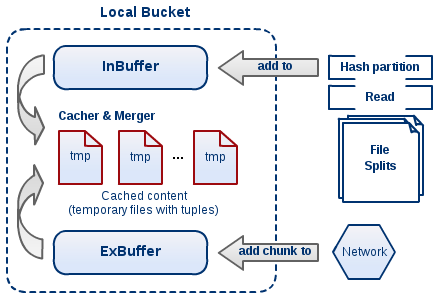
\includegraphics[scale=0.6]{diag4a}
\linebreak
\linebreak
\centering
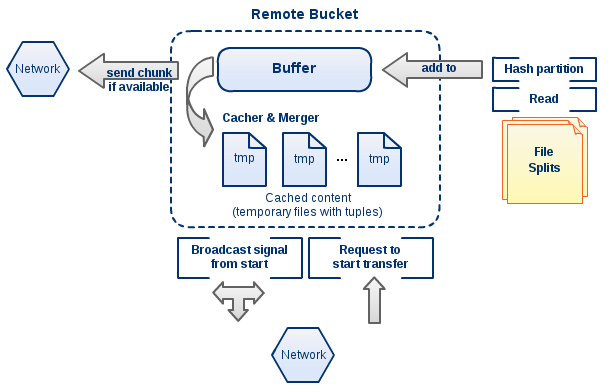
\includegraphics[scale=0.6]{diag4b}
\caption{New local/remote buckets}
\label{fig:diag4}
\end{figure}

% 
\subsubsection*{(3) Double-buffering for writing the results in files}

The last idea refers to writing down the sorted local-bucket (all the triples) into the final result file. This phase uses a \textit{bucketIterator} to iterate over the results. As in turn the iterator uses multiple \textit{removeChunk()} method calls to fetch chunks from the local-bucket, when there are no more triples to iterate/write down. An idea would be to hide the time that the iterator has to wait for merging-up triples from the main memory (buffer) with the ones stored on the disk. Instead we can try to remove/get a chunk that has been already processed and stored in a set of auxiliary buffers in memory (triples ready to be 'served' to the iterator). To implement that, we start a separate thread at the right moment we set the bucket's flag on finished to fill up auxiliary buffers with chunks from the main buffer. When a write is being performed the iterator is called and the chunk is taken directly from the auxiliary buffers instead of waiting for the whole merging. Moreover, when a buffer from the set gets emptied the thread will go on and try to refill it, if there are anymore triples for doing that -- this mechanism of storing buffers that were processed earlier is generally called 'Double-Buffering'. Figure~\ref{fig:diag5} shows how this mechanism was implemented for the \textit{removeChunk()}. 

\begin{figure}
\centering
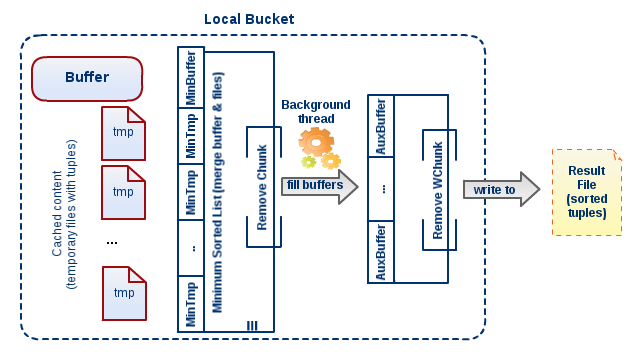
\includegraphics[scale=0.6]{diag5}
\caption{In-background merge-up}
\label{fig:diag5}
\end{figure}

% 
\subsubsection{Results: execution-time}

Test - 8 nodes
\newline \newline
\renewcommand{\arraystretch}{1.2}
{\footnotesize\tt
\begin{tabularx}{\linewidth}{*{10}{c|}}
\cline{2-10}
& SplitSz 
& \multicolumn{3}{c|}{256MB} & \multicolumn{3}{c|}{1GB}  & \multicolumn{1}{c|}{2GB} & \multicolumn{1}{c|}{4GB} \\
\cline{2-10}
& DataSz 
& 21 & 38 & 62 & 21 & 38 & 62 & 62 & 149 \\
\cline{2-10}
& 1
& 2m40.815s & 7m57.255s & 15m41.617s & 3m2.585s & 7m26.847s & 15m52.020s & 16m58.103s & 47m33.350s \\
\cline{2-10}
& 2
& 2m34.868s & 6m15.128s & 15m32.877s & 2m39.325s & 8m52.215s & 15m37.135s & 15m16.995s & 47m29.418s \\
\cline{2-10}
& 3
& 2m30.706s & 6m5.774s & 14m47.793s & 2m43.720s & 5m58.528s & 17m16.021s & 16m24.077s & 47m23.859s \\
\cline{2-10}
& 4
& 2m30.446s & 6m53.190s & 14m49.342s & 2m44.330s & 6m58.543s & 15m51.803s & 15m56.746s & 47m21.741s \\
\cline{2-10}
& 5
& 3m4.606s & 6m43.932s & 15m25.822s & 2m40.153s & 5m13.739s & 17m2.552s & 16m12.159s & 47m26.099s \\
\cline{2-10}
& 6
& 3m9.408s & 6m28.413s & 16m11.942s & 2m40.224s & 5m25.047s & 15m24.170s & 16m31.383s & 47m21.517s \\
\cline{2-10}
& 7
& 2m48.874s & 4m46.725s & 16m25.753s & 2m32.941s & 6m19.333s & 14m18.357s & 16m52.848s & 43m6.666s \\
\cline{2-10}
& 8
& 2m40.238s & 7m25.513s & 15m45.134s & 2m28.537s & 9m11.525s & 15m9.601s & 16m18.642s & 43m55.177s \\
\cline{2-10}
& 9
& 2m30.935s & 6m55.467s & 15m41.847s & 2m33.696s & 7m53.475s & 16m0.388s & 16m25.423s & 46m44.169s \\
\cline{2-10}
& 10
& 2m37.317s & 6m54.436s & 15m38.446s & 2m53.944s & 7m19.787s & 17m15.853s & 16m26.889s & 47m10.179s \\
\cline{2-10}
& Avg (mm.ss)
& 2.7 & 6.63 & 15.59 & 2.69 & 7.05 & 15.97 & 16.3 & 46.54 \\
\cline{2-10}
& Improv. \%
& 7.53 & 13.11 & 1.70 & 11.51 & 12.96 & 10.78 & 7.91 & -NONE- \\
\cline{2-10}
\end{tabularx}

}

\newpage

Test - 12 nodes
\newline \newline
\renewcommand{\arraystretch}{1.2}
{\footnotesize\tt
\begin{tabularx}{\linewidth}{c|c|c|c|c|c|c|c|c|c|l|}
\cline{2-10}
& SplitSz 
& \multicolumn{3}{c|}{256MB} & \multicolumn{3}{c|}{1GB}  & \multicolumn{1}{c|}{2GB} & \multicolumn{1}{c|}{4GB} \\
\cline{2-10}
& DataSz 
& 21 & 38 & 62 & 21 & 38 & 62 & 62 & 149 \\
\cline{2-10}
& 1
& 1m50.679s & 5m31.063s & 13m10.769s & 3m6.879s & 6m13.877s & 14m5.243s & 12m51.575s & 45m31.696s \\
\cline{2-10}
& 2
& 1m52.036s & 4m59.978s & 9m8.194s & 2m58.449s & 5m26.362s & 14m2.959s & 12m43.355s & 42m31.401s \\
\cline{2-10}
& 3
& 2m2.744s & 3m51.152s & 13m4.056s & 2m6.365s & 6m8.137s & 14m6.316s & 12m36.971s & 45m2.317s \\
\cline{2-10}
& 4
& 2m9.747s & 6m20.750s & 12m10.497s & 2m59.096s & 5m30.037s & 12m1.829s & 11m4.499s & 43m29.198s \\
\cline{2-10}
& 5
& 2m5.854s & 3m14.792s & 9m13.899s & 2m0.390s & 6m11.867s & 11m55.725s & 9m10.917s & 42m58.603s \\
\cline{2-10}
& 6
& 2m24.353s & 2m51.950s & 12m23.965s & 2m2.408s & 4m28.531s & 13m57.812s & 11m45.212s & 43m7.404s \\
\cline{2-10}
& 7
& 1m46.429s & 3m38.576s & 12m18.557s & 2m24.491s & 5m40.746s & 14m15.596s & 11m45.168s & 43m53.767s \\
\cline{2-10}
& 8
& 1m43.859s & 5m3.728s & 10m57.489s & 2m12.176s & 4m19.665s & 14m13.373s & 10m49.813s & 42m42.329s \\
\cline{2-10}
& 9
& 2m1.370s & 5m43.489s & 12m3.150s & 2m8.212s & 3m48.096s & 12m38.087s & 11m22.283s & 43m25.376s \\
\cline{2-10}
& 10
& 2m2.946s & 4m35.691s & 12m38.006s & 2m5.706s & 5m45.697s & 13m15.133s & 12m35.941s & 44m49.665s \\
\cline{2-10}
& Avg (mm.ss)
& 2 & 4.57 & 11.7 & 2.4 & 5.34 & 13.44 & 11.66 & 43.74 \\
\cline{2-10}
& Improv. \%
& 10.31 & 26.53 & 7.14 & 21.31 & 19.46 & 6.99 & 2.43 & -NONE- \\
\cline{2-10}
\end{tabularx}

}

Test - 16 nodes
\newline \newline
\renewcommand{\arraystretch}{1.2}
{\footnotesize\tt
\begin{tabularx}{\linewidth}{*{10}{c|}}
\cline{2-10}
& SplitSz 
& \multicolumn{3}{c|}{256MB} & \multicolumn{3}{c|}{1GB}  & \multicolumn{1}{c|}{2GB} & \multicolumn{1}{c|}{4GB} \\
\cline{2-10}
& DataSz 
& 21 & 38 & 62 & 21 & 38 & 62 & 62 & 149 \\
\cline{2-10}
& 1
& 1m41.969s & 3m49.298s & 13m55.218s & 2m36.927s & 6m4.237s & 10m39.667s & 8m48.566s & 40m37.759s \\
\cline{2-10}
& 2
& 1m40.338s & 3m47.789s & 13m19.358s & 2m1.960s & 5m24.346s & 12m40.292s & 9m17.997s & 37m54.868s \\
\cline{2-10}
& 3
& 1m39.998s & 2m55.300s & 13m40.155s & 2m2.099s & 5m38.308s & 13m1.947s & 7m57.156s & 38m20.263s \\
\cline{2-10}
& 4
& 1m32.664s & 4m10.906s & 13m12.273s & 1m49.085s & 6m28.060s & 13m17.127s & 9m3.974s & 37m43.711s \\
\cline{2-10}
& 5
& 1m31.912s & 3m23.316s & 10m36.658s & 2m2.151s & 4m41.135s & 11m55.222s & 6m19.858s & 41m32.575s \\
\cline{2-10}
& 6
& 1m30.868s & 3m20.186s & 14m11.719s & 2m17.648s & 5m0.436s & 13m16.737s & 6m2.039s & 40m37.573s \\
\cline{2-10}
& 7
&  1m31.340s & 5m5.723s & 13m0.218s & 2m19.167s & 5m35.444s & 12m24.751s & 4m13.467s & 37m54.181s \\
\cline{2-10}
& 8
& 1m26.041s & 5m1.699s & 12m32.280s & 2m27.565s & 6m4.404s & 12m32.675s & 9m56.222s & 37m59.779s \\
\cline{2-10}
& 9
& 1m28.403s & 4m23.519s & 10m58.033s & 1m59.172s & 4m47.506s & 13m15.030s & 8m57.491s & 37m3.179s \\
\cline{2-10}
& 10
& 1m43.837s & 3m41.606s & 12m5.290s & 2m11.033s & 4m25.160s & 11m9.291s & 6m46.095s & 34m2.013s \\
\cline{2-10}
& Avg (mm.ss)
& 1.56 & 3.95 & 12.74 & 2.17 & 5.41 & 12.41 & 7.73 & 38.36 \\
\cline{2-10}
& Improv. \%
& 7.14 & 4.13 & -NONE- & -NONE- & -NONE- & 12.11 & 20.23 & 1.31 \\
\cline{2-10}
\end{tabularx}

}

\newpage

Speedup test: average on the best 10 execution-times (mm.ss), see Figure~\ref{fig:speedup}
\newline \newline
\renewcommand{\arraystretch}{1.2}
{\footnotesize\tt
\begin{tabularx}{\linewidth}{*{7}{c|}}
\cline{2-7}
& DataSz|SplitSz
& \multicolumn{5}{c|}{38GB|256MB} \\
\cline{2-7}
& NumNodes
& 1 & 2 & 4 & 8 & 16 \\
\cline{2-7}
& Ajira
& 41.33 & 27.03 & 14.24 & 8.27 & 5.24 \\
\cline{2-7}
& Ajira-Research
& 38.54s & 22.52 & 14.3 & 8.1 & 4.02 \\
\cline{2-7}
\end{tabularx}

}

\begin{figure}
\centering
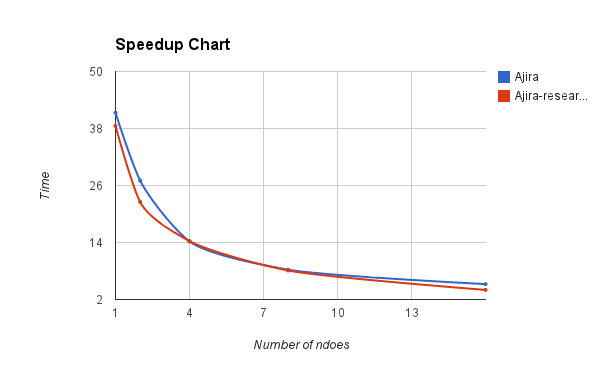
\includegraphics[scale=0.6]{speedup}
\caption{Speedup-chart for Ajira[blue] \& Ajira-Research[red]}
\label{fig:speedup}
\end{figure}

% 
\subsubsection*{Discussion}

\subsection{Future work}

For future work I propose the following developments:

\begin{itemize}
	\item \textit{Moving to processes.} One idea is to implement an option/feature that allows specifying how many 'instances' of PartitionToNodes to run locally and how many remotely on other nodes (following the Apache design model, i.e multiple mappers on same node). Example: if 1 node has 4 x QuadCore CPUs --- in total we can run 8 instances at least (maximum 16), 2 local instances on every node (given the fact that one instance makes highly use of multi-threading is fair enough to start only 2 processes per node).
	\item \textit{Thread synchronization.} In Ajira framework we use threads for background processing and all the methods tend to be globally synchronized for avoiding race conditions on the data structures. This adds a significant overhead to the application, because the access to the data structures becomes coarse grained. A solution for that is to use fine-grained/free-locks data structures or a similar mechanism with double buffering. 
	\item \textit{Fine-grained file splitting.} For the current Ajira version we coarsely split the data set between nodes. That means we consider an entire file when we decide where to send it (in what split collection), for further computation, instead of splitting the file in multiple pieces (i.e 64MB) and take their sizes into consideration. For small size files (with an order of maximum tens of MB) the coarse grained level works fine, but if the dataset has bigger files in small numbers we can get into an unbalanced situation.
	\item \textit{Data sampling.} In the current state of Ajira, the output of a distributed sorting application is not globally ordered. It means that we still have to merge each result file in order to get a full sorted data set from the start to its end. Instead of that, a well known method to achieve global ordering and also a fair data balancing is to perform a previous step called \textit{sampling}. As a state-of-the-art idea is to rely on a Trie (a prefix tree) based algorithm with a depth level fixed in such a way that will assure you enough granularity to equally balance the key partitions to all your nodes. After you have computed the tree you will use that as a tuple partitioner instead of a hash algorithm in your normal data computation. An example of a Trie based sampling algorithm applied with Hadoop Map-Reduce can be seen at \cite{terasort}.
\end{itemize}

\subsection{Conclusions}
% CHAPTER_END